% Course project report, Group 2 (Trustworthy Machine Learning, Fall 2026), in the NeurIPS 2025 style (preprint option).
% Compile: pdflatex report ; bibtex report ; pdflatex report ; pdflatex report   (or: latexmk -pdf -jobname=Group2_report report)
% Numbers: ../five_models/results.json (scores in %, paired-bootstrap differences in points) and
% ../five_models/stopping_failures.json (Figure 1).
\documentclass{article}

\usepackage[preprint]{neurips_2025}
\usepackage[utf8]{inputenc}
\usepackage[T1]{fontenc}
\usepackage[hidelinks]{hyperref}
\usepackage{url}
\usepackage{booktabs}
\usepackage{amsfonts,amsmath}
\usepackage{microtype}
\usepackage{graphicx}
\usepackage{array}

% This is a course report, not a NeurIPS submission: replace the style's venue notice.
\makeatletter
\renewcommand{\@noticestring}{Course project report, Trustworthy Machine Learning (Fall 2026), Virginia Tech.}
\makeatother

\newcommand{\passk}[1]{pass@#1}

\title{Data Selection and Training Budget for Reasoning\\Supervised Fine-Tuning of Qwen2.5-3B-Instruct}

\author{%
  Hanze Li \quad Sijie Chen \quad Yuan Zhou \quad Yiming Liang \\
  Group 2, Trustworthy Machine Learning (Fall 2026) \\
  Virginia Tech, Blacksburg, VA, USA
}

\begin{document}

\maketitle

\begin{abstract}
Supervised fine-tuning (SFT) on long chain-of-thought (CoT) demonstrations is a common way to improve the reasoning ability
of small language models, but which demonstrations to train on remains an open design choice. We study this choice for
Qwen2.5-3B-Instruct under a fixed budget of 15K examples drawn from a 100K subset of AceReason-1.1-SFT. We design a
label-free selection pipeline that combines domain filtering, exact deduplication, length filtering to the training
context, and stratified sampling over data source and solution length. On eight math and science benchmarks, our final
model, trained for five epochs on the selected data, achieves a macro \passk{8} of 59.0\% on the six leaderboard benchmarks,
compared with 53.9\% for the base model and 54.9\% for a random-selection baseline, as well as the highest macro \passk{1}
(26.9\%). Our analysis shows that the gains stem primarily from fewer generations being truncated at the 32,768-token limit.
\end{abstract}

\section{Introduction}

Distilling long CoT traces from strong reasoning models into smaller models through SFT has become a standard recipe for
improving mathematical reasoning~\citep{openthoughts,acereason11,s1}. Small models, however, do not benefit uniformly from
such data: they often fail to absorb long reasoning traces~\citep{li2025small}, and long-reasoning models are prone to
overthinking, i.e., generating excessively long reasoning~\citep{chen2024overthinking}. The choice of training examples
therefore matters when the data budget is limited.

In this project~\citep{course}, we fine-tune Qwen2.5-3B-Instruct~\citep{qwen25} on 15K examples selected from a 100K subset
of AceReason-1.1-SFT~\citep{acereason11}, whose responses are long CoT traces generated by DeepSeek-R1, and ask whether a
principled selection of the 15K examples outperforms random selection. Our contributions are as follows:
\begin{itemize}
  \item We design a label-free data selection pipeline that requires no model inference and yields complete, deduplicated,
        and length-balanced math demonstrations (Section~\ref{sec:data}).
  \item Our final model, trained for five epochs on the selected data, improves macro \passk{8} by 5.1 points over the base
        model and macro \passk{1} by 2.3 points over the random baseline; both 95\% confidence intervals exclude zero
        (Section~\ref{sec:results}).
  \item We identify truncation at the generation limit as the dominant failure mode of the fine-tuned models and separate the
        contributions of data selection and training budget (Section~\ref{sec:results}).
\end{itemize}

\section{Data selection strategy}\label{sec:data}

\paragraph{Random baseline.} The training pool contains 100,000 examples, of which 67,432 are math and 32,568 are code. The
random baseline samples 15,000 examples uniformly with a fixed seed and no filtering. Of these, 556 exceed the 16,384-token
training context and are truncated, so their final answers are removed from the training target.

\paragraph{Selected set.} Our pipeline applies four steps in order. First, \emph{domain filtering} keeps only math examples,
since all target benchmarks are math or science and code traces are off-target. Second, \emph{exact deduplication} removes
repeated prompts (7,730 among the math examples) and keeps the first occurrence, which increases prompt
diversity~\citep{acereason11}. Third, \emph{length filtering} keeps only examples whose full conversation fits the
16,384-token context under the Qwen chat template (removing 2,292), so that every training target ends with its final answer
and end-of-turn token. Fourth, \emph{stratified sampling} with proportional allocation draws 15,000 of the 57,410 remaining
examples over strata defined by data source (NuminaMath-CoT and OpenMathReasoning) and total-length band (up to 4K, 4--8K, and
8--16K tokens), which preserves the source mix and the range of difficulty implied by solution length. The resulting set
contains 107.6M training tokens per epoch (113.4M for the random set), has a median length of 6.5K tokens, and shares 2,252
examples with the random set.

\paragraph{Design rationale.} The pipeline follows evidence that a small, curated fine-tuning set can match or exceed a larger
unfiltered one, both for alignment~\citep{lima} and for reasoning~\citep{s1,limo}, as well as the question filtering and
source mixing studied in data recipes for reasoning models~\citep{openthoughts}. It uses no model scoring, embeddings, or
answer keys. A data-contamination check found six pool prompts that match a benchmark question verbatim; one of them falls
into each 15K set and is kept and disclosed rather than removed from only one arm.

\section{Experimental setup}

\paragraph{Training.} Both models are trained with full-parameter SFT in LLaMA-Factory~\citep{llamafactory}, using DeepSpeed
ZeRO-3~\citep{zero}, FlashAttention-2~\citep{flashattn2}, and the Liger fused linear cross-entropy kernel~\citep{liger}; the
loss is computed on response tokens only. Table~\ref{tab:hparams} lists the hyperparameters. The final model is trained for
three epochs and then resumed from the epoch-3 weights, optimizer, and scheduler states for two additional epochs on a
five-epoch cosine schedule.

\begin{table}[t]
\caption{Training hyperparameters of the final model and the random baseline.}\label{tab:hparams}
\centering\small
\begin{tabular}{@{}>{\raggedright\arraybackslash}p{3.0cm}>{\raggedright\arraybackslash}p{5.3cm}>{\raggedright\arraybackslash}p{4.7cm}@{}}
\toprule
& \textbf{Final model} & \textbf{Random baseline} \\
\midrule
Training data & Selected 15K (107.6M tokens/epoch) & Random 15K (113.4M tokens/epoch) \\
Epochs (steps) & 5 (9,375) & 3 (5,625) \\
Learning rate & $5\times10^{-6}$, cosine, no warmup; epochs 4--5 decay from $1.7\times10^{-6}$ to 0 & $5\times10^{-6}$, cosine, no warmup \\
Tokens seen & 538.2M & 338.8M \\
Hardware (time) & 4$\times$L40S (8.6\,h) + 4$\times$A100 (4.4\,h) & 4$\times$L40S (9.2\,h) \\
\midrule
Base model & \multicolumn{2}{l}{Qwen2.5-3B-Instruct, full-parameter SFT, loss on response tokens} \\
Optimizer & \multicolumn{2}{l}{AdamW, $\beta=(0.9,0.999)$, weight decay 0, gradient clipping 1.0} \\
Global batch size & \multicolumn{2}{l}{8 (4 GPUs $\times$ micro-batch 1 $\times$ gradient accumulation 2)} \\
Max.\ sequence length & \multicolumn{2}{l}{16,384 tokens, Qwen chat template} \\
Precision, kernels & \multicolumn{2}{l}{bf16, DeepSpeed ZeRO-3, FlashAttention-2, Liger kernel} \\
\bottomrule
\end{tabular}
\end{table}

\paragraph{Benchmarks and metrics.} We evaluate on AIME24, MATH-500, CN-Math 2024, Kaoyan, AMC, Minerva, OlympiadBench, and
GPQA using the course evaluation harness, which generates with vLLM~\citep{vllm} and grades the last boxed answer by symbolic
equivalence. For each question, we draw $n=8$ samples with temperature 0.6, top-$p$ 0.95, and a maximum of 32,768 generated
tokens. We report \passk{8}, which counts a question as solved if any of the eight samples is correct (the \passk{k} metric
of \citet{codex} with $k=n$), and \passk{1}, the mean per-sample accuracy. The macro score averages, with equal weight, the six
leaderboard benchmarks available to us (CN-Math 2024, Kaoyan, AMC, Minerva, OlympiadBench, and GPQA); AIME24 and MATH-500 are
reported but excluded from the leaderboard average. We report differences between models in percentage points with 95\%
confidence intervals (CIs) from a paired bootstrap over questions ($B=2000$), in which the eight samples of each question are
kept together~\citep{efron1993,miller2024}.

\section{Results and analysis}\label{sec:results}

\begin{table}[t]
\caption{Results on the eight benchmarks (\passk{8} and \passk{1}, \%). $N$: number of questions; $^{*}$: benchmark included
in the macro average.}\label{tab:results}
\centering\small
\begin{tabular}{@{}lcccccc@{}}
\toprule
& \multicolumn{2}{c}{\textbf{Base}} & \multicolumn{2}{c}{\textbf{Random 15K}} & \multicolumn{2}{c}{\textbf{Final model}} \\
\cmidrule(lr){2-3}\cmidrule(lr){4-5}\cmidrule(l){6-7}
Benchmark ($N$) & \passk{8} & \passk{1} & \passk{8} & \passk{1} & \passk{8} & \passk{1} \\
\midrule
AIME24 (30) & 16.7 & 7.1 & 33.3 & 7.1 & 23.3 & 7.5 \\
MATH-500 (500) & 84.0 & 65.3 & 88.4 & 64.7 & 87.8 & 66.0 \\
CN-Math 2024$^{*}$ (30) & 36.7 & 10.4 & 33.3 & 7.9 & 33.3 & 10.4 \\
Kaoyan$^{*}$ (199) & 54.8 & 21.9 & 65.3 & 29.2 & 67.8 & 29.8 \\
AMC$^{*}$ (40) & 65.0 & 39.1 & 57.5 & 34.4 & 77.5 & 38.1 \\
Minerva$^{*}$ (272) & 45.2 & 28.7 & 47.1 & 25.5 & 45.6 & 27.3 \\
OlympiadBench$^{*}$ (675) & 49.8 & 27.7 & 52.6 & 27.8 & 53.8 & 30.1 \\
GPQA$^{*}$ (198) & 71.7 & 29.4 & 73.7 & 23.0 & 75.8 & 25.8 \\
\midrule
Macro ($^{*}$) & 53.9 & 26.2 & 54.9 & 24.6 & \textbf{59.0} & \textbf{26.9} \\
\bottomrule
\end{tabular}
\end{table}

\begin{figure}[t]
\centering
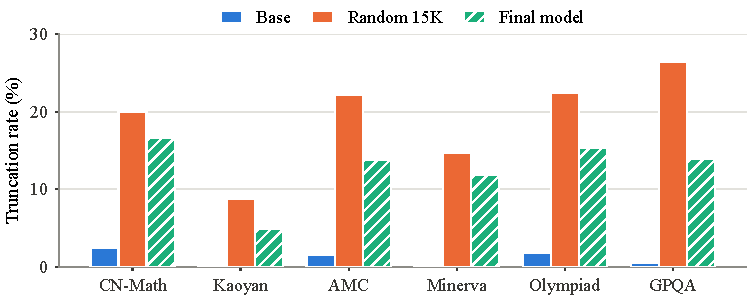
\includegraphics[width=0.9\textwidth]{fig_cutoff.pdf}
\caption{Truncation rate, i.e., the share of samples that reach the 32,768-token generation limit, on the six leaderboard
benchmarks.}
\label{fig:cutoff}
\end{figure}

\paragraph{Main results.} Table~\ref{tab:results} summarizes the results. Fine-tuning on randomly selected data yields only a
marginal improvement over the base model (+1.1 points in macro \passk{8}, 95\% CI [$-4.2$, 6.2]) and even reduces macro
\passk{1} by 1.6 points. In contrast, our final model improves macro \passk{8} by 5.1 points over the base model (95\% CI
[0.9, 9.5]), the only improvement over the base model that is significant at the 95\% level, and outperforms the random
baseline by 4.0 points in \passk{8} (95\% CI [$-0.4$, 8.6]) and by 2.3 points in \passk{1} (95\% CI [0.9, 3.8]). The gains are
most pronounced on Kaoyan (+13.1 points in \passk{8} over the base model) and AMC (+20.0 points over the random baseline). On
AIME24, which is excluded from the macro average, the final model underperforms the random baseline by 10.0 points, i.e.,
three of 30 questions.

\paragraph{Truncation explains most of the gain.} We find that truncation at the generation limit is the dominant failure mode
of the fine-tuned models. Both fine-tuned models generate CoT traces 8--16$\times$ longer than the base model, consistent with
the overthinking behavior reported for long-reasoning models~\citep{chen2024overthinking}. As shown in
Figure~\ref{fig:cutoff}, 8.7--26.5\% of the samples of the random baseline reach the 32,768-token limit before producing an
answer, and such truncated samples are almost never correct (0--4\% accuracy). Our final model reduces the truncation rate on
every leaderboard benchmark, to 4.8--16.7\%, while the accuracy of completed samples remains comparable (e.g., 35.5\% vs.\
35.2\% on OlympiadBench and 30.9\% vs.\ 29.6\% on Minerva). Reducing truncation therefore translates directly into higher
\passk{1} and \passk{8}. We hypothesize that two factors contribute. First, length filtering ensures that every training target
is a complete solution that ends with an answer, whereas 556 targets in the random set are truncated. Second, longer training
further suppresses run-on generation: on a held-out set of 200 pool questions that appear in neither training set, the
truncation rate of the selected run decreases from 55\% after epoch 1 to 24\% after epoch 3 and 16\% after epoch 5. This is
consistent with \citet{acereason11}, who report that SFT accuracy on this data family keeps improving up to about five epochs.

\paragraph{Data selection or training budget?} Because the final model is trained for five epochs and the random baseline for
three, the comparison conflates data selection and training budget. Under an equal budget of three epochs, the selected data
achieves a macro \passk{8} of 56.6\% and \passk{1} of 24.4\%, a gain of 1.6 points in \passk{8} over the random baseline
(95\% CI [$-2.4$, 5.6]) that lies within question-sampling noise. We therefore attribute the improvement of the final model to
the combination of the selected data and the longer training, rather than to data selection alone.

\paragraph{Limitations.} Each configuration is trained once, so our confidence intervals capture question-sampling variance
but not training-seed variance. The five-epoch schedule was chosen after the three-epoch results were known, and the final
model is selected on the benchmarks on which it is reported; AIME25, which is part of the course leaderboard but not available
to us, is the only unseen test set. All training data come from the provided pool. Adding external data is allowed but would
require decontamination against the benchmarks; short, curated reasoning sets~\citep{s1,limo}, which suit small
students~\citep{li2025small}, and science data for GPQA are natural extensions. Additional selection methods we evaluated,
including a learning-progress selector, are documented in the full report in our repository.

\section{Conclusion}

We studied training-data selection for reasoning SFT of Qwen2.5-3B-Instruct under a 15K-example budget. A label-free
selection of complete, deduplicated math demonstrations, combined with five epochs of training, raises macro \passk{8} from
53.9\% to 59.0\% and macro \passk{1} from 26.2\% to 26.9\%, outperforming the random baseline (54.9\% and 24.6\%). Our analysis
suggests that, for a 3B student trained on long CoT data, reducing truncated generations is a key lever for improving
reasoning performance. Code, configurations, and evaluation logs are available at
\url{https://github.com/yuan-zhou-git/Course_Project_Trustworthy_ML}, and the final model and datasets at
\url{https://huggingface.co/yuan-zhou-hf}.

\bibliographystyle{plainnat}
\bibliography{refs}

\end{document}
